\documentclass{article}
%\usepackage[cyr]{aeguill}
\usepackage[utf8]{inputenc}
\usepackage[T1]{fontenc}
\usepackage[francais]{babel}
\usepackage{amsmath}
\usepackage{fancyhdr}
\usepackage{amsfonts}
\usepackage{makeidx}         
\title{Projet GM4 : Programme de détection de spam}
\usepackage[pdftex]{graphicx}
\author{Jean Prost \and Edouard Gouteux \and Lucas Potin} 
 
\begin{document}
\maketitle
 
% une série de blocs comme celui qui suit
\section{Modélisation UML}

\subsection{Présentation de la méthode}

La méthode est expliquée sur le site\\

Les classes java utilisées pour l'implémentation de la méthode : \\
- Scanner : classe relative au traitement du texte, contient les méthodes permettant de remplir les différents types de table de hachage. \\
- Predicteur : classe qui permet de prédire si un mail est un spam ou non. \\
- Mail : classe contenant le mail sous forme d'un fichier texte.\\
- Corpus : Ensemble de mail. \\

2 types de Table de Hachage  :\\
- table contenant les mails (Non Spam / Spam).\\
- table contenant les probabilités basée sur l'apparition des jetons dans les mails spam/non spam.\\

\subsection{Diagramme des cas d'utilisation}

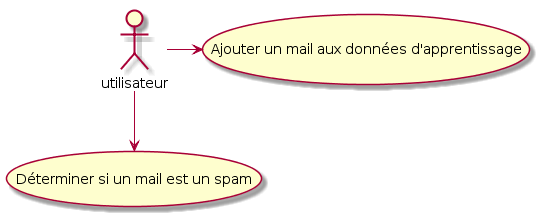
\includegraphics[scale=0.6]{diag_usecase.png}

\subsection{Diagramme de séquence}
On considère la situation ou, l'utilisateur souhaite connaître la probabilité estimée que son mail soit un spam.

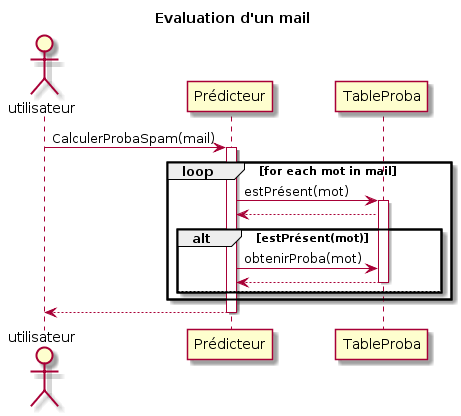
\includegraphics[scale=0.7]{diag_sequence.png}

\subsection{Diagramme de classe}

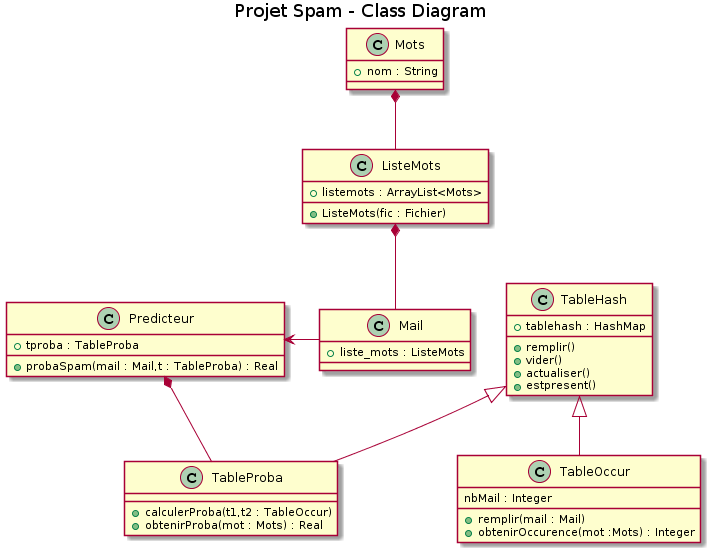
\includegraphics[scale=0.5]{diag_classe.png}





 
\end{document}